\documentclass[convert]{standalone}

\usepackage{tikz}
\usepackage{graphicx}
\pagestyle{empty}

% INT_AY22_L25-Fig02_Parallel_wires.png

\begin{document}
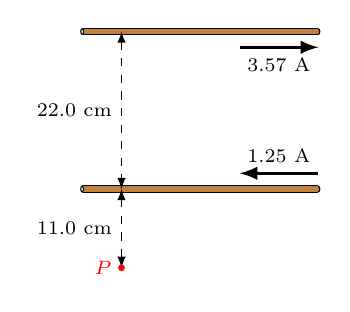
\begin{tikzpicture}[> = latex, font = \scriptsize]

	% Definition
	
	\def\L{1.2}		% Position of marked points
	
	% Top current wire with direction
	
	\draw [double = brown, double distance = 2 pt] (-1.5, 1) -- (1.5, 1);
	\filldraw [brown] (1.5, 1.035) arc (90 : -90 : 0.5 pt and 1 pt) -- cycle;
	\filldraw [white] (-1.5, 1.035) arc (90 : -90 : 0.5 pt and 1 pt) -- cycle;
	\draw (1.5, 1.035) arc (90 : -90 : 0.5 pt and 1 pt);
	\draw (-1.5, 1) ellipse (0.5 pt and 1 pt);
	
	\draw [->, very thick] (0.5, 0.8) -- node [midway, below] {3.57 A} (1.5, 0.8);
	
	% Bottom current wire with direction
	
	\draw [double = brown, double distance = 2 pt] (-1.5, -1) -- (1.5, -1);
	\filldraw [brown] (1.5, -1.035) arc (-90 : 90 : 0.5 pt and 1 pt) -- cycle;
	\filldraw [white] (-1.5, -1.035) arc (-90 : 90 : 0.5 pt and 1 pt) -- cycle;
	\draw (1.5, -1.035) arc (-90 : 90 : 0.5 pt and 1 pt);
	\draw (-1.5, -1) ellipse (0.5 pt and 1 pt);
	
	\draw [->, very thick] (1.5, -0.8) -- node [midway, above] {1.25 A} (0.5, -0.8);
	
	% Distance indicators
	
	\draw [dashed, <->] (-1, 1) -- node [left] {22.0 cm} (-1, -1);
	\draw [dashed, <->] (-1, -1) -- node [left] {11.0 cm} (-1, -2);
	
	\filldraw [red] (-1, -2) circle (1 pt) node [left] {$P$};

\end{tikzpicture}
\end{document}